
\section{Is every individual happy after equilibrium?}
As it is shown in the previous section, equilibrium is not always reached within 10000 generations, or at all. 
But when it does, it is natural to question whether every individual is happy and how happy they are. 
To answer this question, we ran 500 simulations for each happiness rule ranging from 0 to 1 with increments of 0.01 and we calculated what the average, maximum and minimum happiness of the population is for each happiness rule. 
We ran the simulations for an $8\times 8$ bord and 40 individuals and 20 per type. 
The result is shown in figure \ref{happyhappy}.\\
\\
In figure \ref{happyhappy}, we observed that the minimum happiness is almost always equal to or greater than the happiness rule, which means that every individual is happy after the equilibrium. 
We also saw that maximum happiness is always 1, which means there is always one invididual who has all his/her neighbours of the same type. 
Furthermore, we see that the average happiness is always closer to the maximum happiness than to the minimum happiness and that at around a happiness rule of 0.8, we see that every individual has happiness 1. 
This implies that happiness 0.8 guarantees full segregation.\\
\\
It is not very surprising that every individual is happy after the equilibrium, since it would otherwise mean that one individual is unable to find a place that better meets his/her desire. 
On a board with 24 empty spaces, this does not seem very likely. 
Another remarkable result is that figure \ref{happyhappy} shows the minimum happiness is higher than the happiness rule and that the average happiness is closer to 1 if the happiness rule higher than around 0.8. 
At the first glance this might seems impossible because the heavy requirement of being happy, but on the other hand, it shows that the strong 'need' for segregation actually leads to higher happiness.
\begin{figure}[h!]
    \centering
    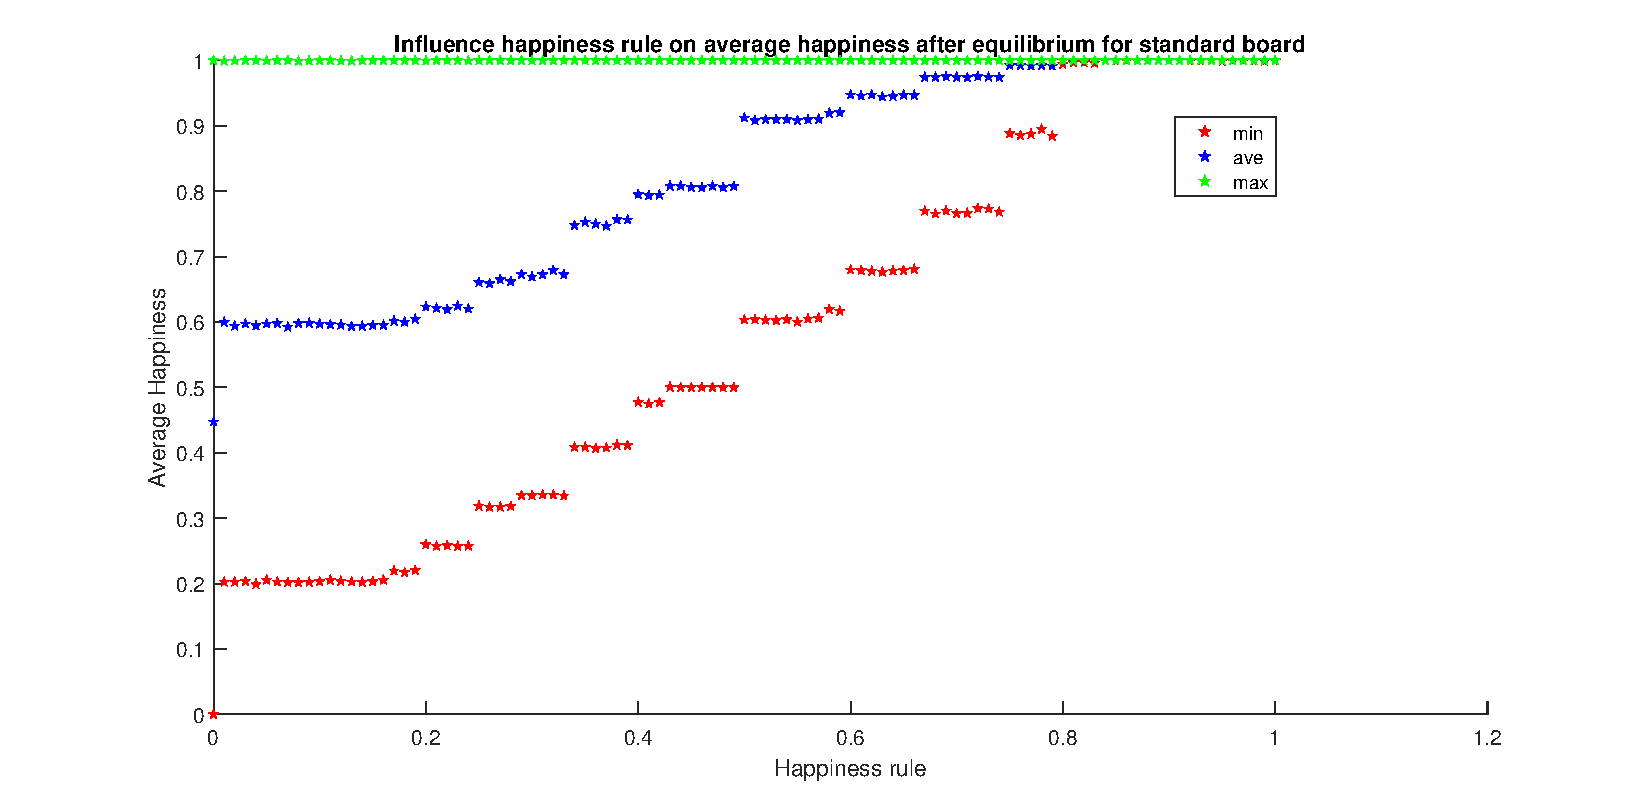
\includegraphics[width=0.9\textwidth]{happinessregel-gemhappinesseind-2.pdf}
    \caption{Influence of happiness rule on the happiness of the individuals. The green graph shows the maximal happiness, the blue graph shows the average happiness and the red graph shows the minimal happiness}
    \label{happyhappy}
\end{figure}
\\
Just to illustrate that the variance of every above calculated average happiness is practically zero, we only selected Happiness Rule 1/3 as an example and made a histogram in figure \ref{minhappy}. 
In figure \ref{minhappy}, we see that the probability of every individual is happy is practically 1.
\newpage
\begin{figure}[H]
    \centering
    \begin{subfigure}{0.8\textwidth}
        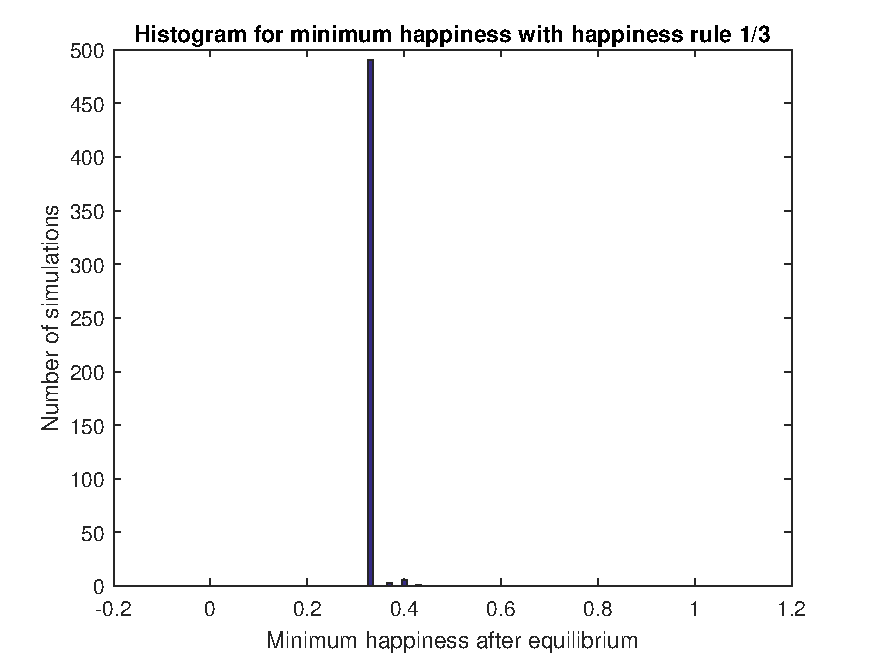
\includegraphics[width=\textwidth]{histogram_min_happiness_een_derde}
    \caption{Histogram for minimum happiness after 500 simulations with HR=1/3 }
    \label{minhappy}
    \end{subfigure}
\end{figure}
%Ik plaats hier random text om ervoor te zorgen dat dingen goedgaan met invoegen gelieve aan te passen.
